% ================================================================================================ capítulo 4
\chapter{Modo educativo}\label{cap:educativo}

\begin{resumen}
\textbf{En este capítulo:} cómo está armado el modo educativo, qué enseña cada lección, cómo usar los datos de ejemplo o
los de un video de la clase, y algunas ideas para dar una clase con él.
\end{resumen}

Medir el seeing es, en el fondo, un ejercicio de estadística: miles de cuadros, cada uno con una distancia un poco
distinta, y una pregunta sobre qué tan dispersas están. El modo educativo aprovecha eso. Cada cuadro del video es un
dato, y con esos datos se aprende a hacer un histograma, a calcular una media y una desviación estándar, a reconocer la
campana de Gauss, a estimar un error y a desconfiar de los datos atípicos. Lo pensamos para colegios y para cursos
introductorios de universidad: no hace falta saber nada de astronomía para empezar.

\captura{edu_bienvenida.png}{La bienvenida del modo educativo, con sus tres caminos.}

El menú de la izquierda tiene tres grupos:
\begin{itemize}
\item \textbf{La estrella}: por qué titilan las estrellas, cómo funciona el truco de los dos orificios y un simulador
de turbulencia. Es la motivación física, contada con animaciones.
\item \textbf{Estadística}: nueve lecciones y una prueba final.
\item \textbf{Tu video}: el mismo flujo del modo medición (capítulo~\ref{cap:medicion}), con explicaciones extra en cada
paso y el historial con el nombre \menu{Mis mediciones}.
\end{itemize}

\section{La estrella}

\textbf{¿Por qué titilan?} Una animación de una moneda en el fondo de una piscina que parece moverse cuando el agua se
agita, y otra de la luz de una estrella que cruza capas de aire de distinta temperatura. Con ellas se entiende que la
estrella no se mueve: es el aire el que dobla la luz.

\captura{edu_titilan.png}{«¿Por qué titilan las estrellas?».}

\textbf{Los dos huequitos.} El principio del DIMM con dos animaciones lado a lado: la máscara con la luz entrando por
dos caminos y lo que ve la cámara. Con \campo{Hacer temblar el telescopio}, los dos puntos se mueven juntos y la
distancia entre ellos casi no cambia; al subir la \campo{Turbulencia}, cada punto baila por su lado y la distancia sí
cambia. Abajo, cinco tarjetas resumen cómo grabar un video propio.

\captura{edu_dimm.png}{«El truco de los dos huequitos»: la idea del DIMM en una pantalla.}

\textbf{Simulador.} Una estrella doble que baila con la turbulencia que elijas, mientras el histograma de la distancia se
arma en vivo. Sirve para ver que más turbulencia es una campana más ancha, y que con pocos datos la campana todavía no se
ve.

\section{Las lecciones de estadística}

Todas las lecciones tienen la misma forma, para que el estudiante sepa dónde buscar cada cosa:

\begin{center}\small
\begin{tabularx}{\linewidth}{@{}>{\bfseries\color{acentoosc}}l Y@{}}
Explicación & Un texto corto con la idea, sin fórmulas al principio.\\
Fórmula & La fórmula de la lección, bien escrita.\\
Pruébalo & Dos o tres cosas concretas para hacer con los controles.\\
Gráfica & Responde en vivo a los controles; como todas las gráficas, muestra valores al pasar el cursor.\\
Controles & Deslizadores y casillas, y \boton{CSV…} y \boton{Excel…} para guardar los datos que se ven.\\
Comprueba & Una pregunta de opción múltiple que se responde una sola vez por sesión; las opciones salen en orden al azar.\\
\end{tabularx}
\end{center}

\captura{edu_l3.png}{Lección 3, media y mediana: al agregar datos raros (que caen a un lado elegido al azar) la media se
desplaza y la mediana casi no.}

\begin{table}[H]
\centering\small
\begin{tabularx}{\linewidth}{@{}c l Y@{}}
\toprule
& Lección & Qué se aprende y qué se hace\\
\midrule
1 & Datos y mediciones & Cada cuadro da un dato: 10~s a 60 cuadros por segundo son 600 datos. Se ve la serie en el
tiempo, que sube y baja sin un patrón fijo.\\
2 & El histograma & Ordenar miles de datos en una imagen. Con muy pocos intervalos se pierde el detalle; con muchísimos
aparecen huecos que son solo ruido.\\
3 & Media y mediana & Dos formas del valor típico. Los datos raros arrastran la media; la mediana es robusta.\\
4 & Dispersión & Varianza y desviación estándar. Al mover la turbulencia la campana se ensancha, la media no cambia y
el seeing sí.\\
5 & La distribución normal & La campana de Gauss y la regla 68–95–99,7, con bandas de 1, 2 y 3~σ sobre los datos
reales.\\
6 & Muestras y error de la media & ¿Cuántos cuadros hacen falta? Se toman 1\,000 muestras al azar y se compara la
dispersión real de sus medias con la predicha, $\sigma/\sqrt{n}$.\\
7 & Datos atípicos & Una historia real: 68 cuadros mal medidos entre 8\,484 casi duplicaron $\sigma$. La limpieza con
la MAD la devuelve a su valor.\\
8 & Correlación & El coeficiente $r$: un cuadro se parece al siguiente, pero no a uno de medio segundo después. Incluye
\emph{Cómo leer $r$ en un DIMM}.\\
9 & Laboratorio libre & Histograma, curva normal y banda ±σ de la separación, del movimiento longitudinal o del
transversal, con los cuadros que elijas.\\
10 & Ponte a prueba & Once preguntas de estadística y del experimento, con la explicación de cada respuesta.\\
\bottomrule
\end{tabularx}
\caption{Las lecciones de estadística.}
\end{table}

\captura{edu_l5.png}{Lección 5: la campana de Gauss sobre los datos reales de Altair.}

\subsection{Cómo leer \texorpdfstring{$r$}{r} en un DIMM}

La lección 8 tiene una tarjeta más, \emph{Cómo leer $r$ en un DIMM}, que aplica la correlación a la propia medición:
calcula los tres controles de calidad de la sección~\ref{sec:controles} con los datos de ejemplo o con los de tu video,
los explica uno por uno y termina con un diagnóstico («la turbulencia domina», «hay vibración en una dirección»\ldots).
Es la forma más directa de conectar la estadística de la clase con la calidad de una medición de verdad.

\begin{figure}[H]
\centering
\tcbox[colback=white,colframe=gris!30,boxrule=0.5pt,arc=1.5mm,left=0pt,right=0pt,top=0pt,bottom=0pt,boxsep=0pt]{%
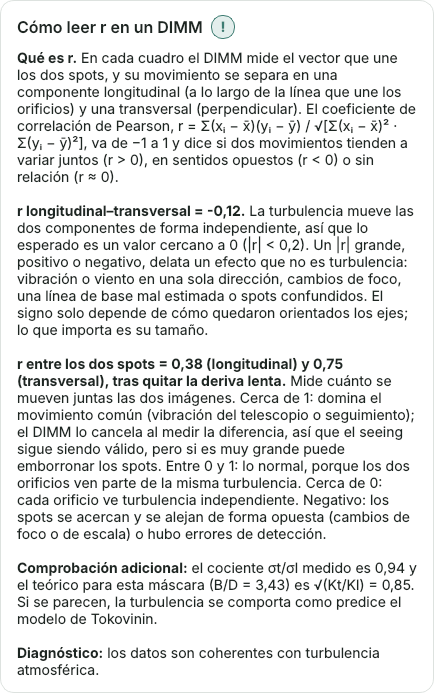
\includegraphics[height=8.5cm]{img/edu_correlacion.png}}
\caption{La tarjeta «Cómo leer $r$ en un DIMM».}
\end{figure}

\section{Los datos: Altair o tu video}

Arriba a la derecha de cada lección está el selector \boton{Altair (ejemplo)} / \boton{Mi video}:
\begin{itemize}
\item \textbf{Altair (ejemplo)} son los 8\,484 cuadros de una medición real de la estrella Altair, grabada por el grupo
con el Celestron 8SE, la Nikon D5600 y la máscara de 4,2/14,4~cm. Vienen con TurbuLENS.
\item \textbf{Mi video} usa el video que se procesó en \menu{Tu video} o, si no hay, el del modo medición. Si
todavía no se ha procesado ninguno, la ficha explica qué hacer y las lecciones siguen con Altair.
\end{itemize}

\section{Ideas para una clase}

\begin{consejo}[Una sesión de dos horas.]
\begin{enumerate}[leftmargin=1.4em]
\item Diez minutos con \menu{¿Por qué titilan?} y \menu{Los dos huequitos}, proyectados, para plantear la pregunta: ¿cómo
se mide algo que tiembla?
\item Las lecciones 1 a 5 en parejas, con los datos de Altair. Cada pareja anota sus respuestas de \emph{Comprueba}
antes de pulsarlas.
\item La lección 7 en grupo: ¿qué habría pasado si nadie revisaba esos 68 cuadros?
\item Si hay telescopio, se graba un video con la máscara (o se usa uno grabado antes) y se procesa en \menu{Tu video}.
Las lecciones se repiten con \boton{Mi video} y se comparan los resultados con los de Altair.
\item \menu{Ponte a prueba} al final, individual.
\end{enumerate}
\end{consejo}

Los resultados de la clase se guardan en \menu{Mis mediciones}, que es el mismo historial del modo medición: un curso
puede ir acumulando mediciones de varias noches y compararlas al final del semestre.
